\chapter {Sequenzdiagramme}
\section{Initialisierung von \projektTitel}
\begin{figure}[h]
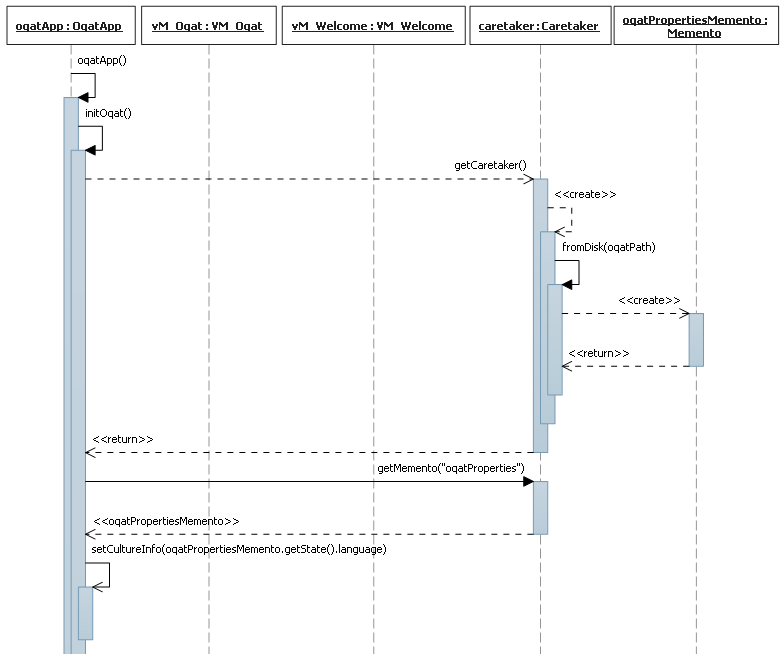
\includegraphics[width=\linewidth]{bilder/Sequenzdiagramm/initOqat1.png}
\label{}
\caption{initOqat1}
\end{figure}

\begin{figure}[h]
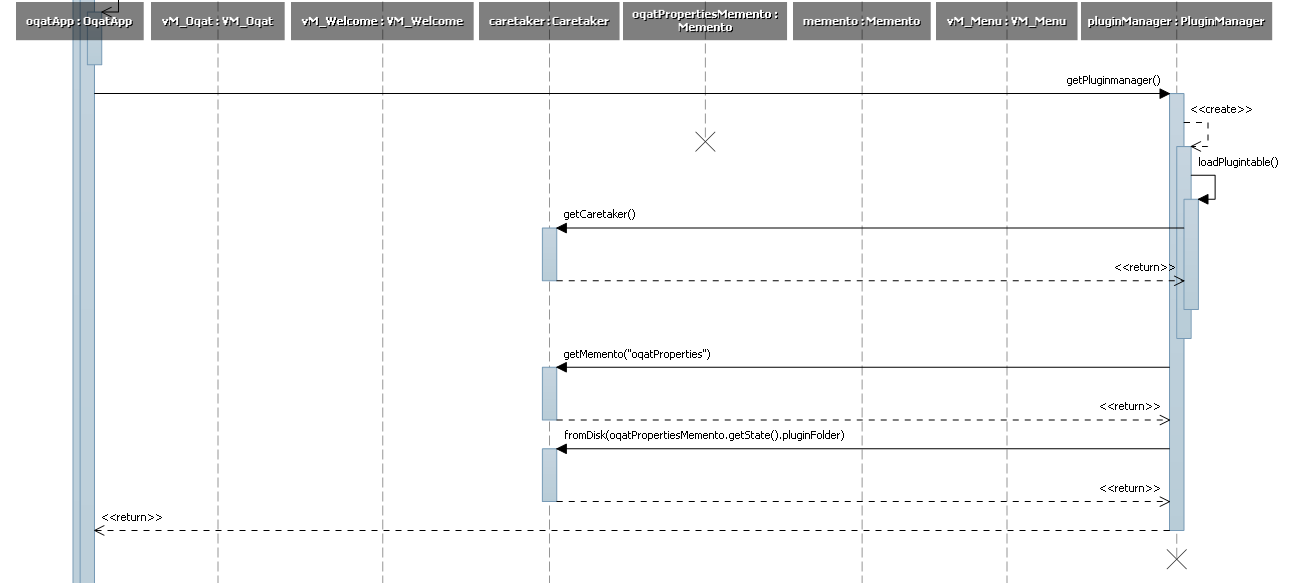
\includegraphics[width=\linewidth]{bilder/Sequenzdiagramm/initOqat2.png}
\label{}
\caption{initOqat2}
\end{figure}

\begin{figure}[h]
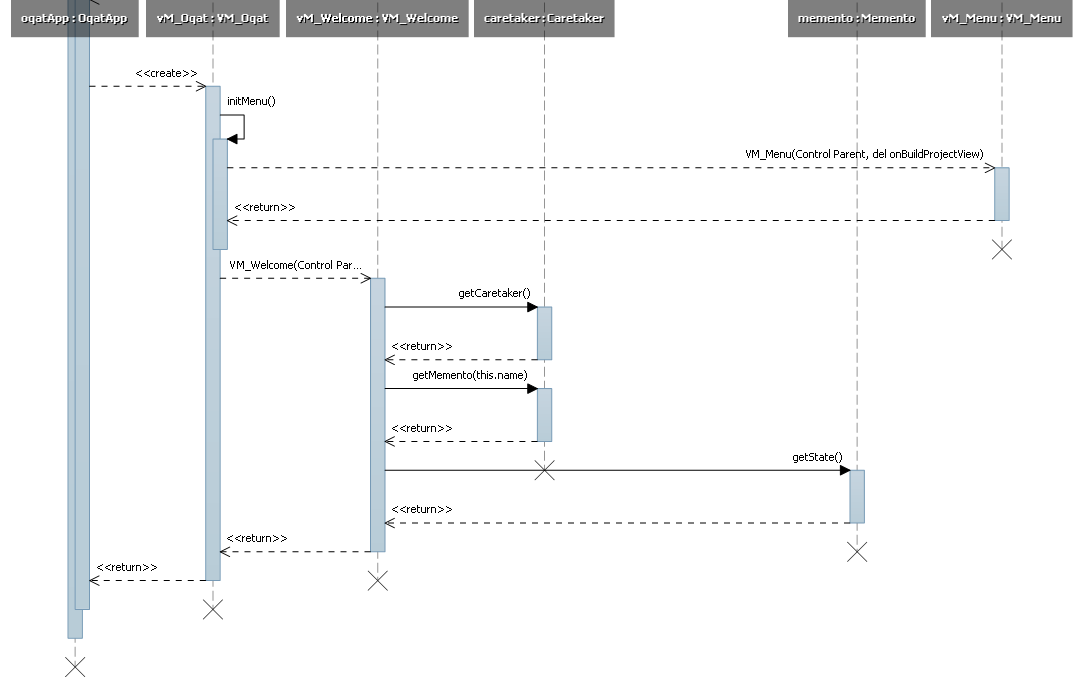
\includegraphics[width=\linewidth]{bilder/Sequenzdiagramm/initOqat3.png}
\label{}
\caption{initOqat3name}
\end{figure}

\section{Initialisierung eines Projekts}
\begin{figure}[h]
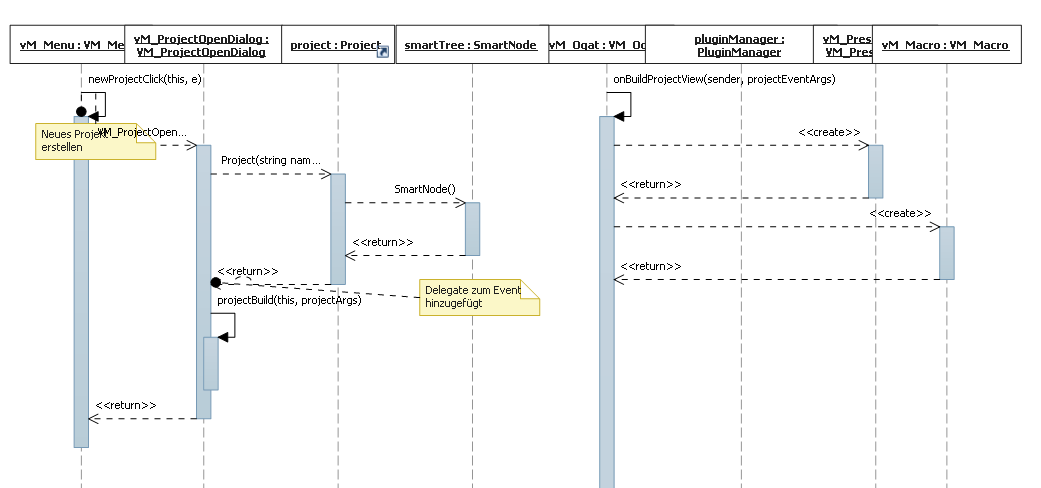
\includegraphics[width=\linewidth]{bilder/Sequenzdiagramm/initProject1.png}
\label{}
\caption{initProject1}
\end{figure}

\begin{figure}[h]
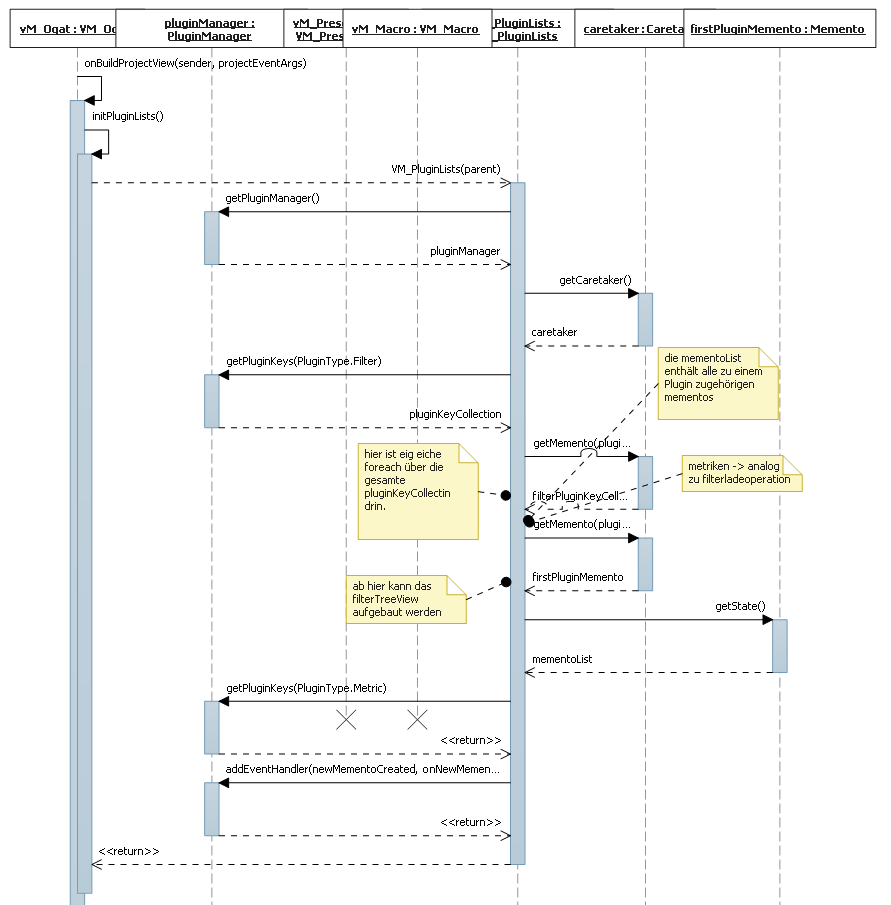
\includegraphics[width=\linewidth]{bilder/Sequenzdiagramm/initProject2.png}
\label{}
\caption{initProject2}
\end{figure}

\newpage
\section{Macro}
\subsection{Macro Filter}
\begin{figure}[h]
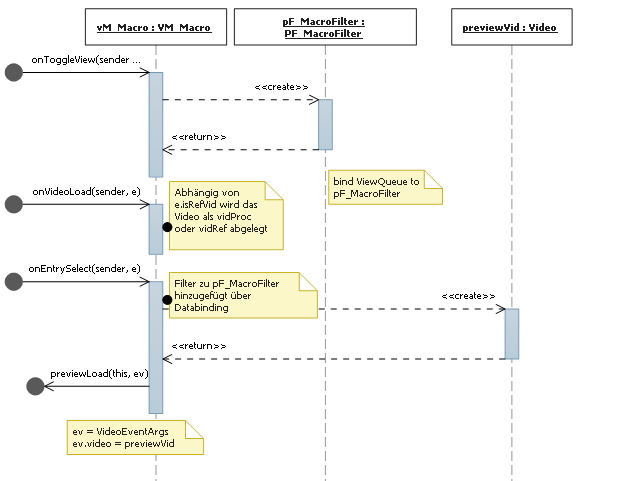
\includegraphics[width=\linewidth]{bilder/Sequenzdiagramm/Macro1.png}
\label{}
\caption{MacroFilter1}
\end{figure}

\begin{figure}[h]
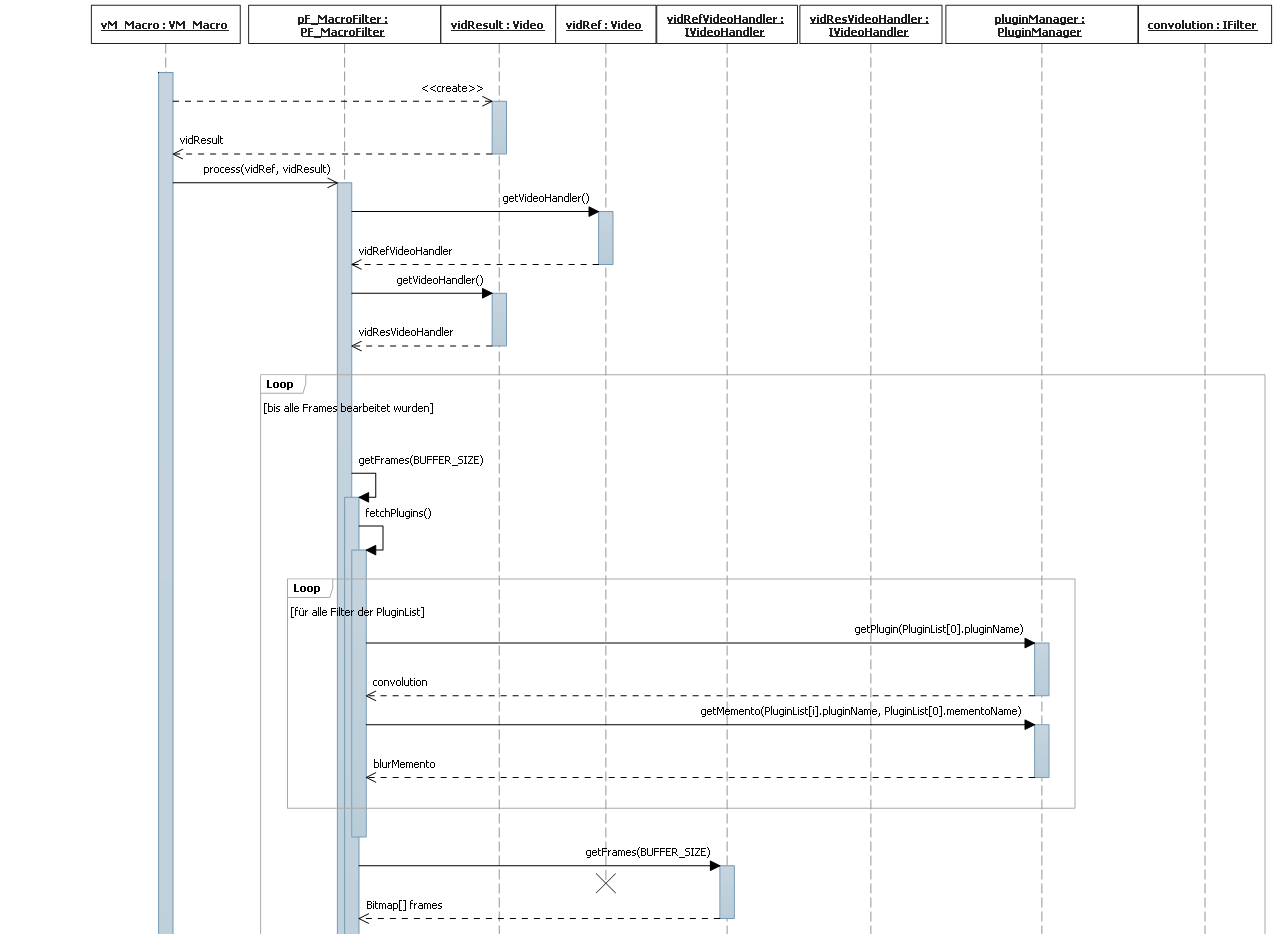
\includegraphics[width=\linewidth]{bilder/Sequenzdiagramm/Macro2.png}
\label{}
\caption{MacroFilter2}
\end{figure}

\begin{figure}[h]
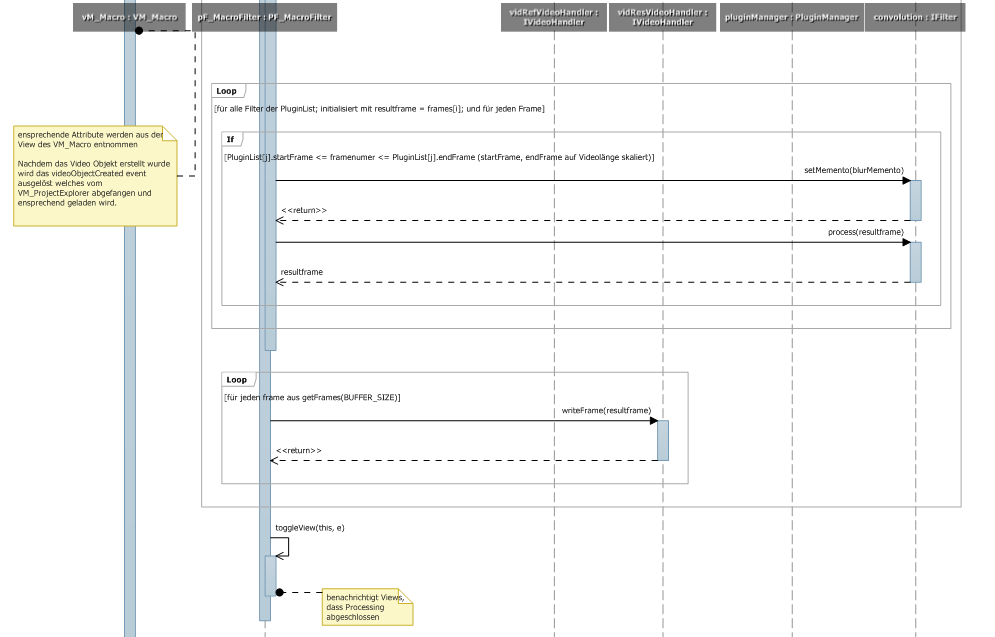
\includegraphics[width=\linewidth]{bilder/Sequenzdiagramm/Macro3.png}
\label{}
\caption{MacroFilter3}
\end{figure}

\subsection{Macro Metric}
\begin{figure}[h]
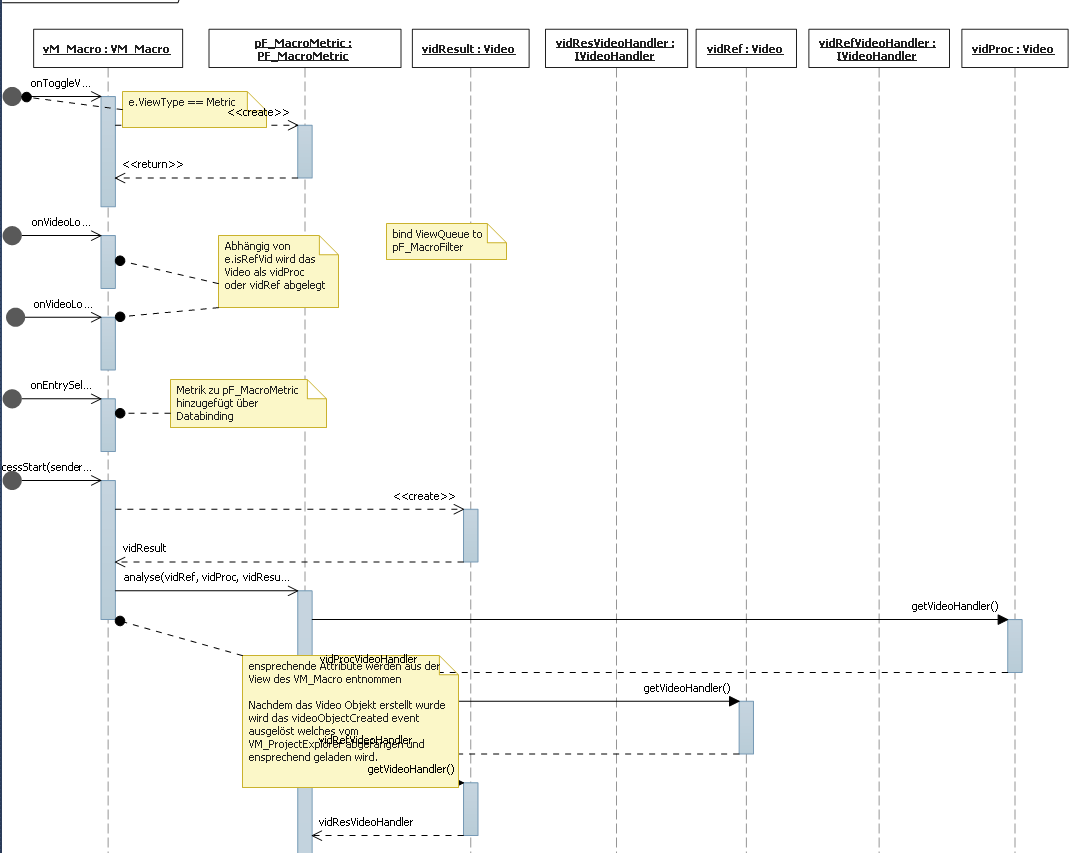
\includegraphics[width=\linewidth]{bilder/Sequenzdiagramm/MacroMetric1.png}
\label{}
\caption{MacroMetric1}
\end{figure}

\begin{figure}[h]
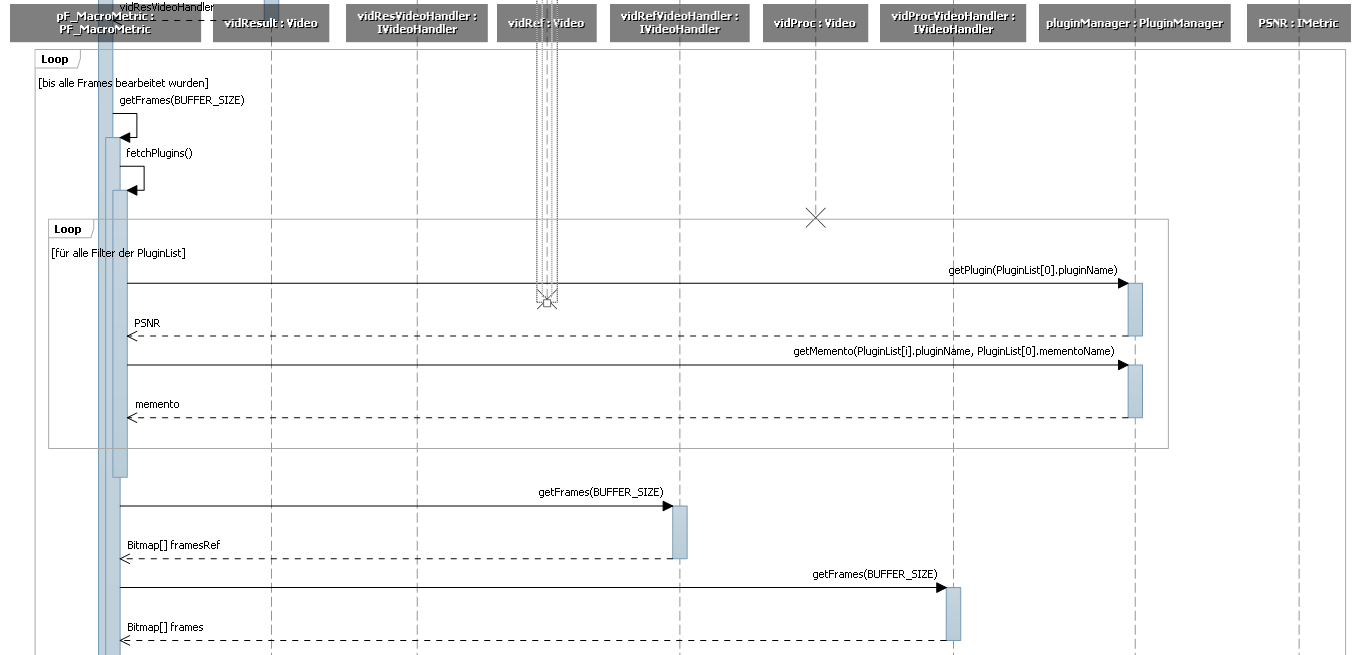
\includegraphics[width=\linewidth]{bilder/Sequenzdiagramm/MacroMetric2.png}
\label{}
\caption{MacroMetric2}
\end{figure}

\begin{figure}[h]
\includegraphics[width=\linewidth]{bilder/Sequenzdiagramm/MacroMetric3.png}
\label{}
\caption{MacroMetric3}
\end{figure}


\section{Video Load}
\begin{figure}[h]
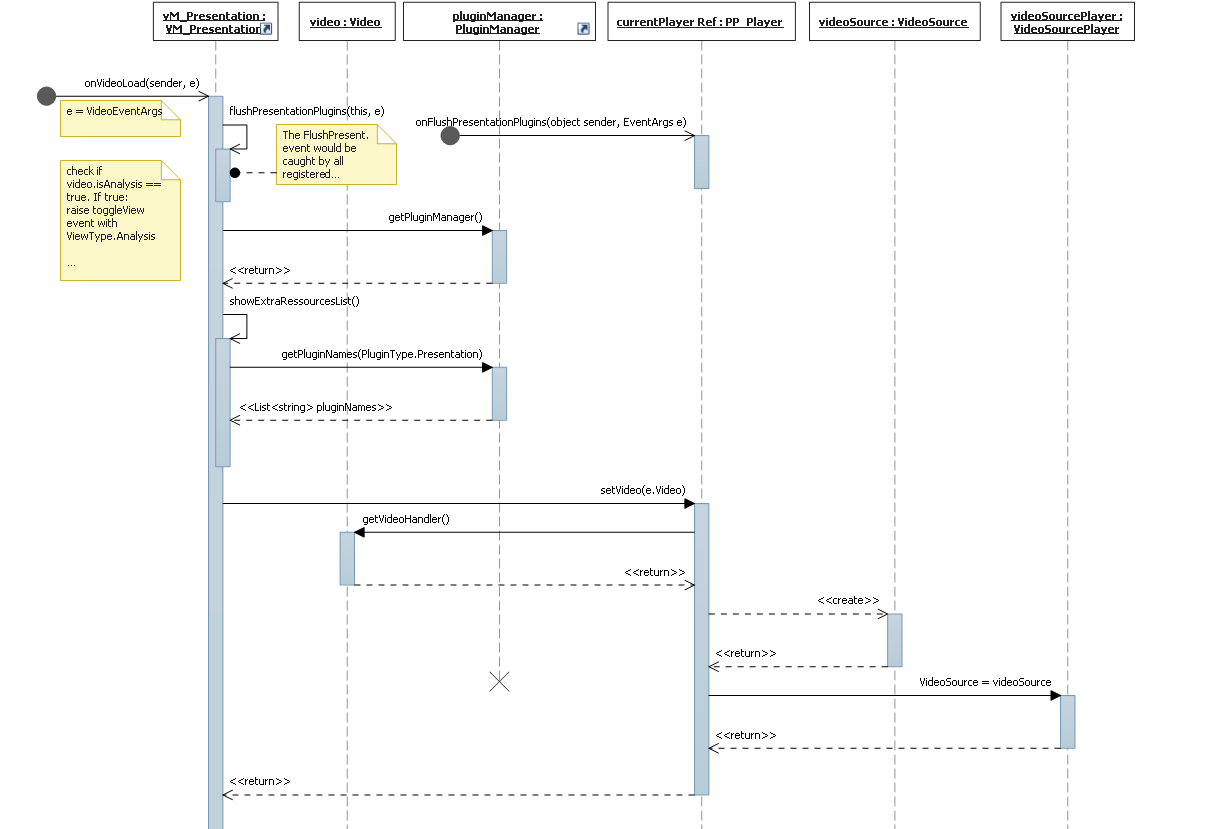
\includegraphics[width=\linewidth]{bilder/Sequenzdiagramm/videoLoad1.png}
\label{}
\caption{videoLoad1}
\end{figure}

\begin{figure}[h]
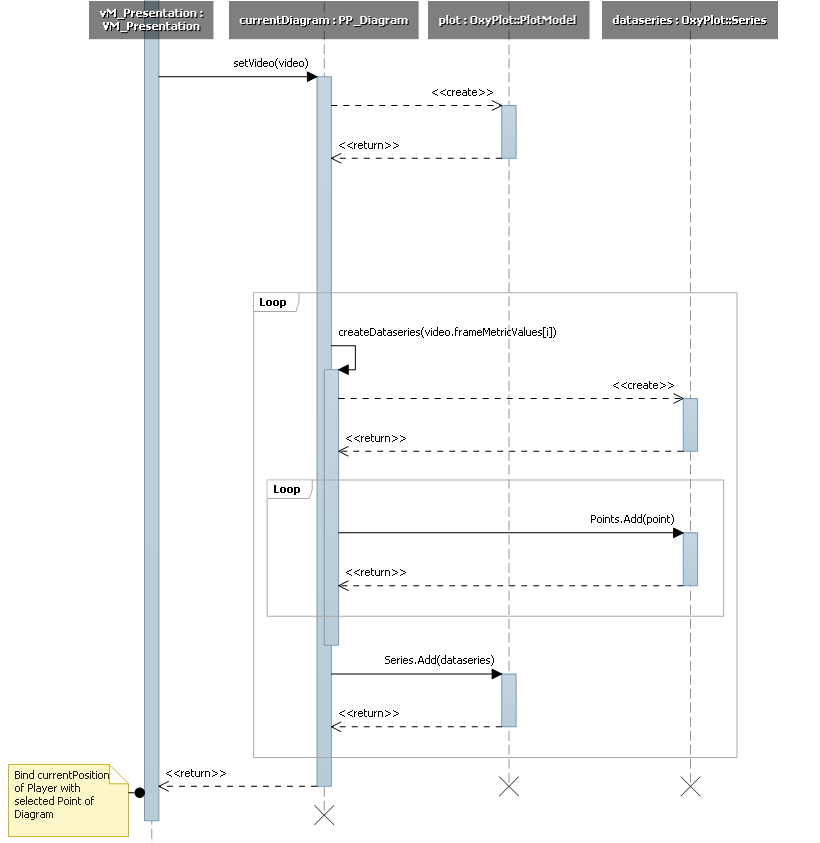
\includegraphics[width=\linewidth]{bilder/Sequenzdiagramm/videoLoad2.png}
\label{}
\caption{videoLoad2}
\end{figure}

\section{Video Extra Ressource}
\begin{figure}[h]
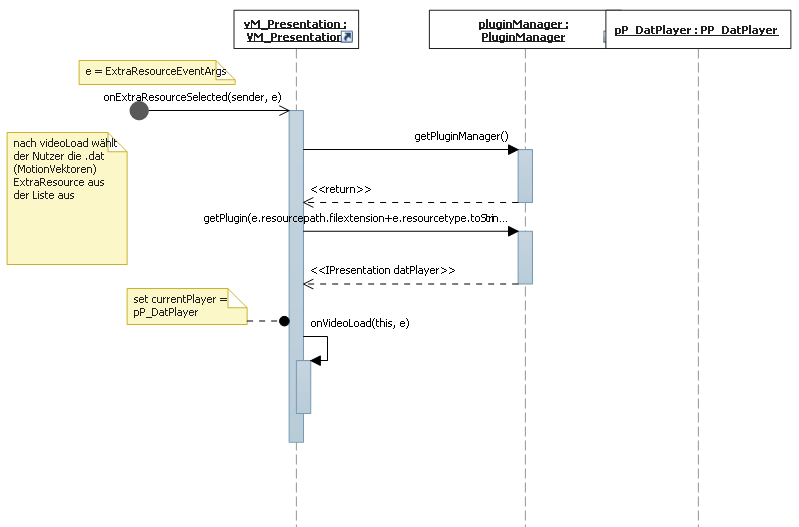
\includegraphics[width=\linewidth]{bilder/Sequenzdiagramm/extraResourcen.png}
\label{}
\caption{extraResourcen}
\end{figure}

\section{vidImport}
\begin{figure}[h]
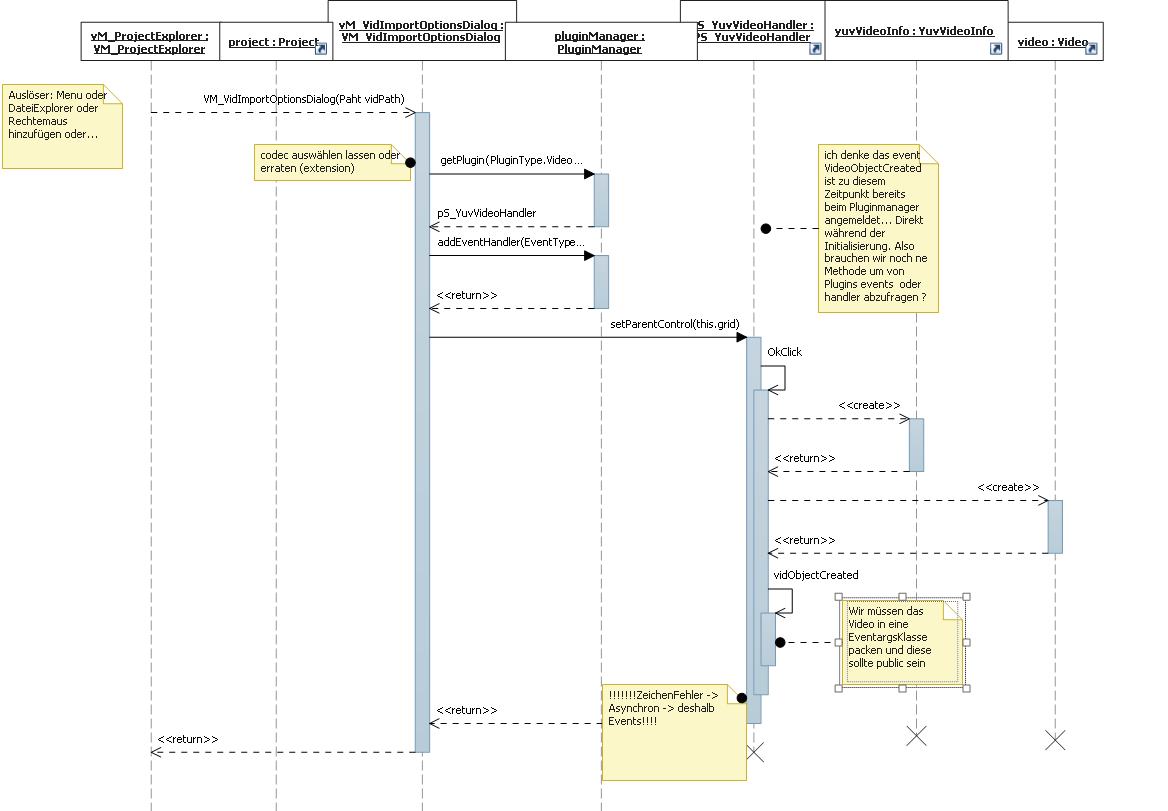
\includegraphics[width=\linewidth]{bilder/Sequenzdiagramm/videoImport.png}
\label{}
\caption{videoImport}
\end{figure}